\documentclass{article}
\usepackage{graphicx} % Required for inserting images

\title{Deep Learning Labwork 1}
\author{2440048 - Thien An NGUYEN}
\date{April 2025}

\begin{document}

\maketitle

\section{Introduction}
In this Labwork, we focus on Gradient Descent, where I implemented the algorithm in Python from scratch.\\
\noindent Gradient Descent is very straightforward, I need to calculate the Gradient of a Function and use the Gradient to find its local (global) minimum (if it exists). Gradient Descent converges to a global minimum in convex functions, while for non-convex functions, it may find a local minimum or a saddle point. Gradient Descent requires the function to be differentiable, and it also depends on the learning rate. Also, if a function has minimums at infinity, Gradient Descent won’t find it.\\
\noindent Of course, there are other ways to find the global (local) minimum of a function, but Gradient Descent finds it iteratively, which is better in high-dimensional or large-scale problems where exact solutions are too costly to compute.

\section{Implementation}
\subsection{The code}
\begin{verbatim}
def gradient_descent(f, x_0, h, L, max_iterations, threshold = 1e-6):
    fx = []
    x_s = []
    for i in range(max_iterations):
        derivative = (f(x_0 + h) - f(x_0 - h)) / (2*h)
        x_a = x_0 - L * derivative
        f_xa = f(x_a)
        fx.append(f_xa)
        x_s.append(x_a)
        print(f"Step {i + 1}: x = {x_a:.6f} | f(x) = {f(x_a):.2f}")

        if abs(f(x_a) - f(x_0)) < threshold:
            break
        x_0 = x_a

    return x_0, fx, x_s
\end{verbatim}

\subsection{Explanation}
My code takes the following inputs:
\begin{itemize}
    \item f: The function that we want to find the minimum of.
    \item x\_0: Our starting point.
    \item h: The step to calculate the gradient (since I used numeric gradient calculation)
    \item L: The learning rate (or the step we want to take follows the Gradient.
    \item max\_iterations: (self explanatory)
    \item threshold: The threshold at which, if the changes after each step are not too big anymore, we stop.
\end{itemize}

\noindent First, the derivative is calculated, then x\_a is an updated version of the position by taking a small step L following the derivative. This will iterate through till all the iterations are done or till the updates are too small.

\section{Experiments}
We will use the $f(x) = x^2$ function for the experiment and experiment with the learning rate of 0.1, 0.3, and 1.2, with the initial x value of 10.

\begin{figure}[ht!]
  \centering
  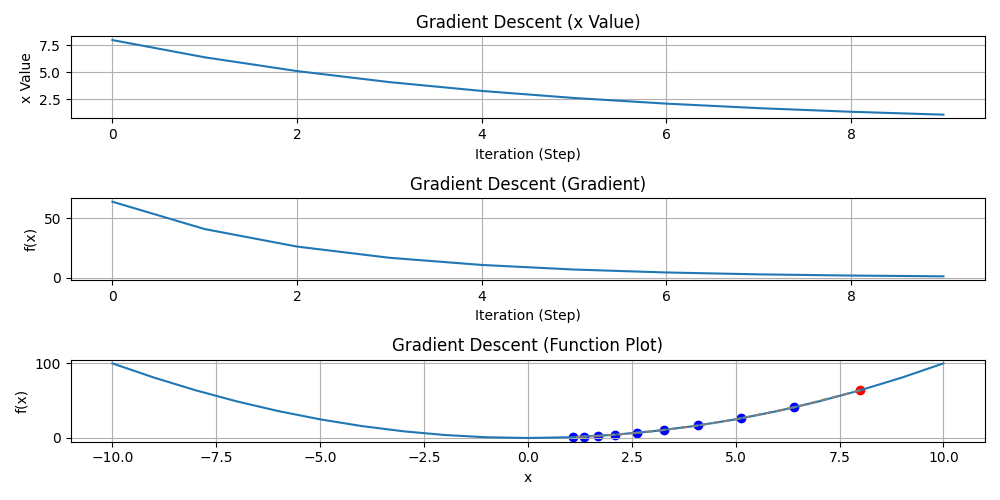
\includegraphics[width=1\textwidth]{images/lab1/gradient_descent_lr(0.1).png}
  \caption{Gradient Descent with Learning Rate 0.1}
  \label{fig:lr_0.1}
\end{figure}

\begin{figure}[ht!]
  \centering
  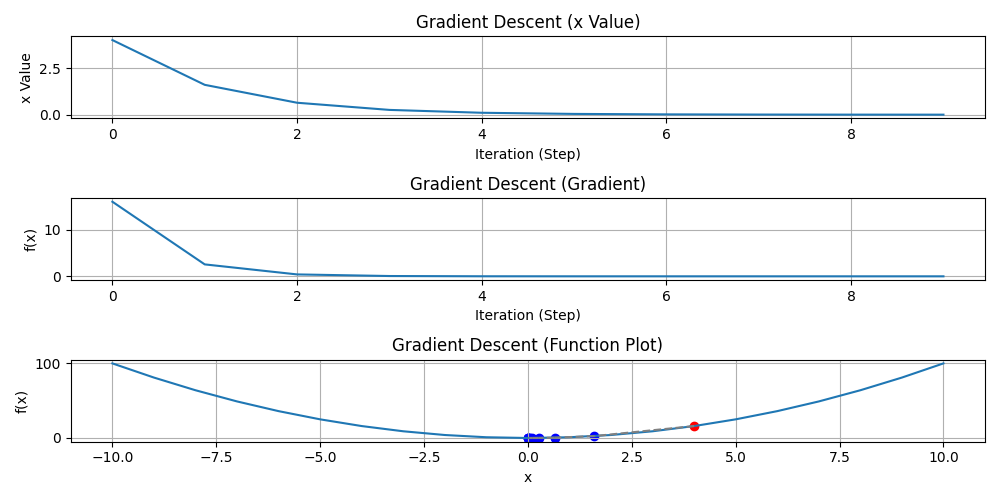
\includegraphics[width=1\textwidth]{images/lab1/gradient_descent_lr(0.3).png}
  \caption{Gradient Descent with Learning Rate 0.3}
  \label{fig:lr_0.3}
\end{figure}

\begin{figure}[ht!]
  \centering
  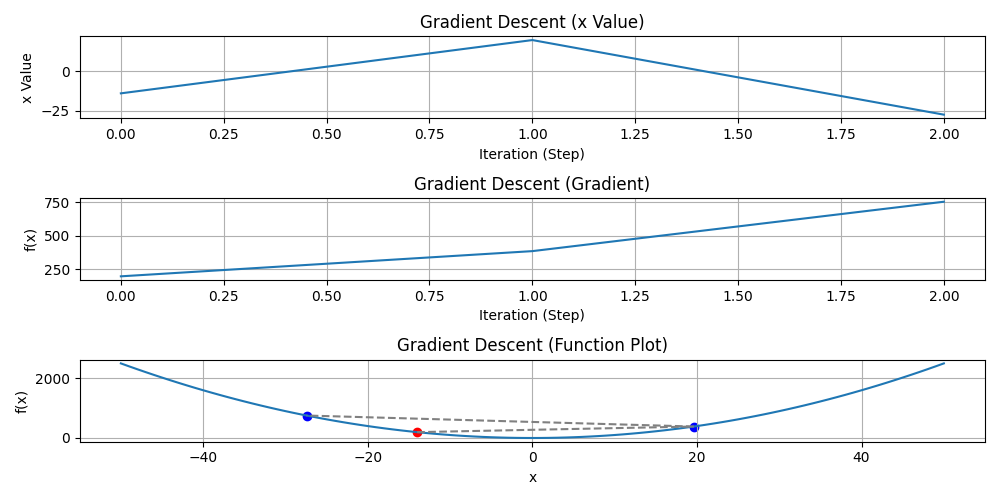
\includegraphics[width=1\textwidth]{images/lab1/gradient_descent_lr(1.2).png}
  \caption{Gradient Descent with Learning Rate 1.2}
  \label{fig:lr_1.2}
\end{figure}

\noindent Here, the red dot visualizes the position after step 1. We can see that Gradient Descent depends a lot learning rate. In the case of a learning rate of 0.1, it converges, but it is a bit slow compared with a learning rate of 0.3. For a learning rate of 1.2, it diverges since it took too big of a step towards the minimum.\\
\noindent The gradient also decreased when the value is closer towards the minimum for the case of 0.1 and 0.3, but for 1,2 the gradient becomes larger cause of the divergence. At the eendnd x converges around 0.

\end{document}
